\chapter{Case study}
\section{Glyph tracking}
The norm in the industry is that CCTV cameras are manually selected depending on needs, usually through using touch screens that display a set of four pictures at once. They are controllable through PTZ, but they are usually only moved to preset locations, by navigating the user interface.

\begin{figure}[ht]
    \centering
    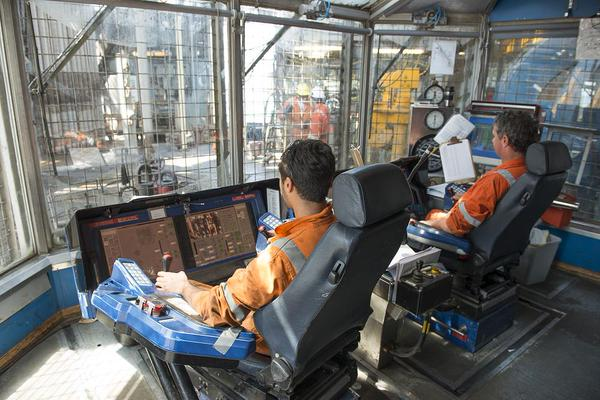
\includegraphics[width=0.8\textwidth]{driller_cabin.jpg}
    \caption{Modern driller cabin. Source:\cite{}}
    \label{fig:}
\end{figure}
\FloatBarrier

\subsection{Design of the computer vision algorithm}


\subsection{Analysis of dataset for robustness in weather conditions}
Based on work done in the project thesis, a Python program using OpenCV 2 was created. Its purpose was to analyse pictures captured over the span of a year, from the MHWirth test tower located at Dvergsnes, Kristiansand.
\begin{equation}
58h 08min 18.3sec N 8h 04min 17.6sec E
\end{equation}

The dataset was gathered using another Python program written and deployed around christmas 2014, which at 15-minute intervals, captured images from a handful of CCTV cameras in the tower and stored them on a local server.

Located at various locations in the fifty meters tall test tower, the idea was that weather impacts would be strong.

As the CCTV cameras have built-in low-light mode, a period during the night is considered too dark for the algorithm to detect the glyph.

The program that gathered the pictures was running without supervision. A result of this was that some gaps of several days in the dataset exists.

Initially, all the pictures were stored as lossless 24-bit RGB Portable Network Graphics. However, after a few months, the amount of data being gathered was filling up the server storage. It was then decided to continue the data gathering using JPEG, which would cut the required storage space close to $\frac{1}{5}$ of the space required with PNG-24

\begin{equation}
\frac{pictures}{camera}=365 days\cdot 24\frac{h}{day}\cdot 4\frac{pics}{h}=35040
\end{equation}

\section{Tubular detection in fingerboard}
Drilling pipes and risers, commonly called tubulars, are used to drill deep into the earth.

These tubulars need to be stored in between their use in the drilling process. The most common method for short-term to mid-term storage is in groups of a few units in a machine called fingerboard, a part of the pipe handling equipment on a drilling rig.

The circularity of a circle can be described using the Heywood circularity factor. This factor can be used to narrow feature detection.

\begin{figure}[ht]
    \centering
    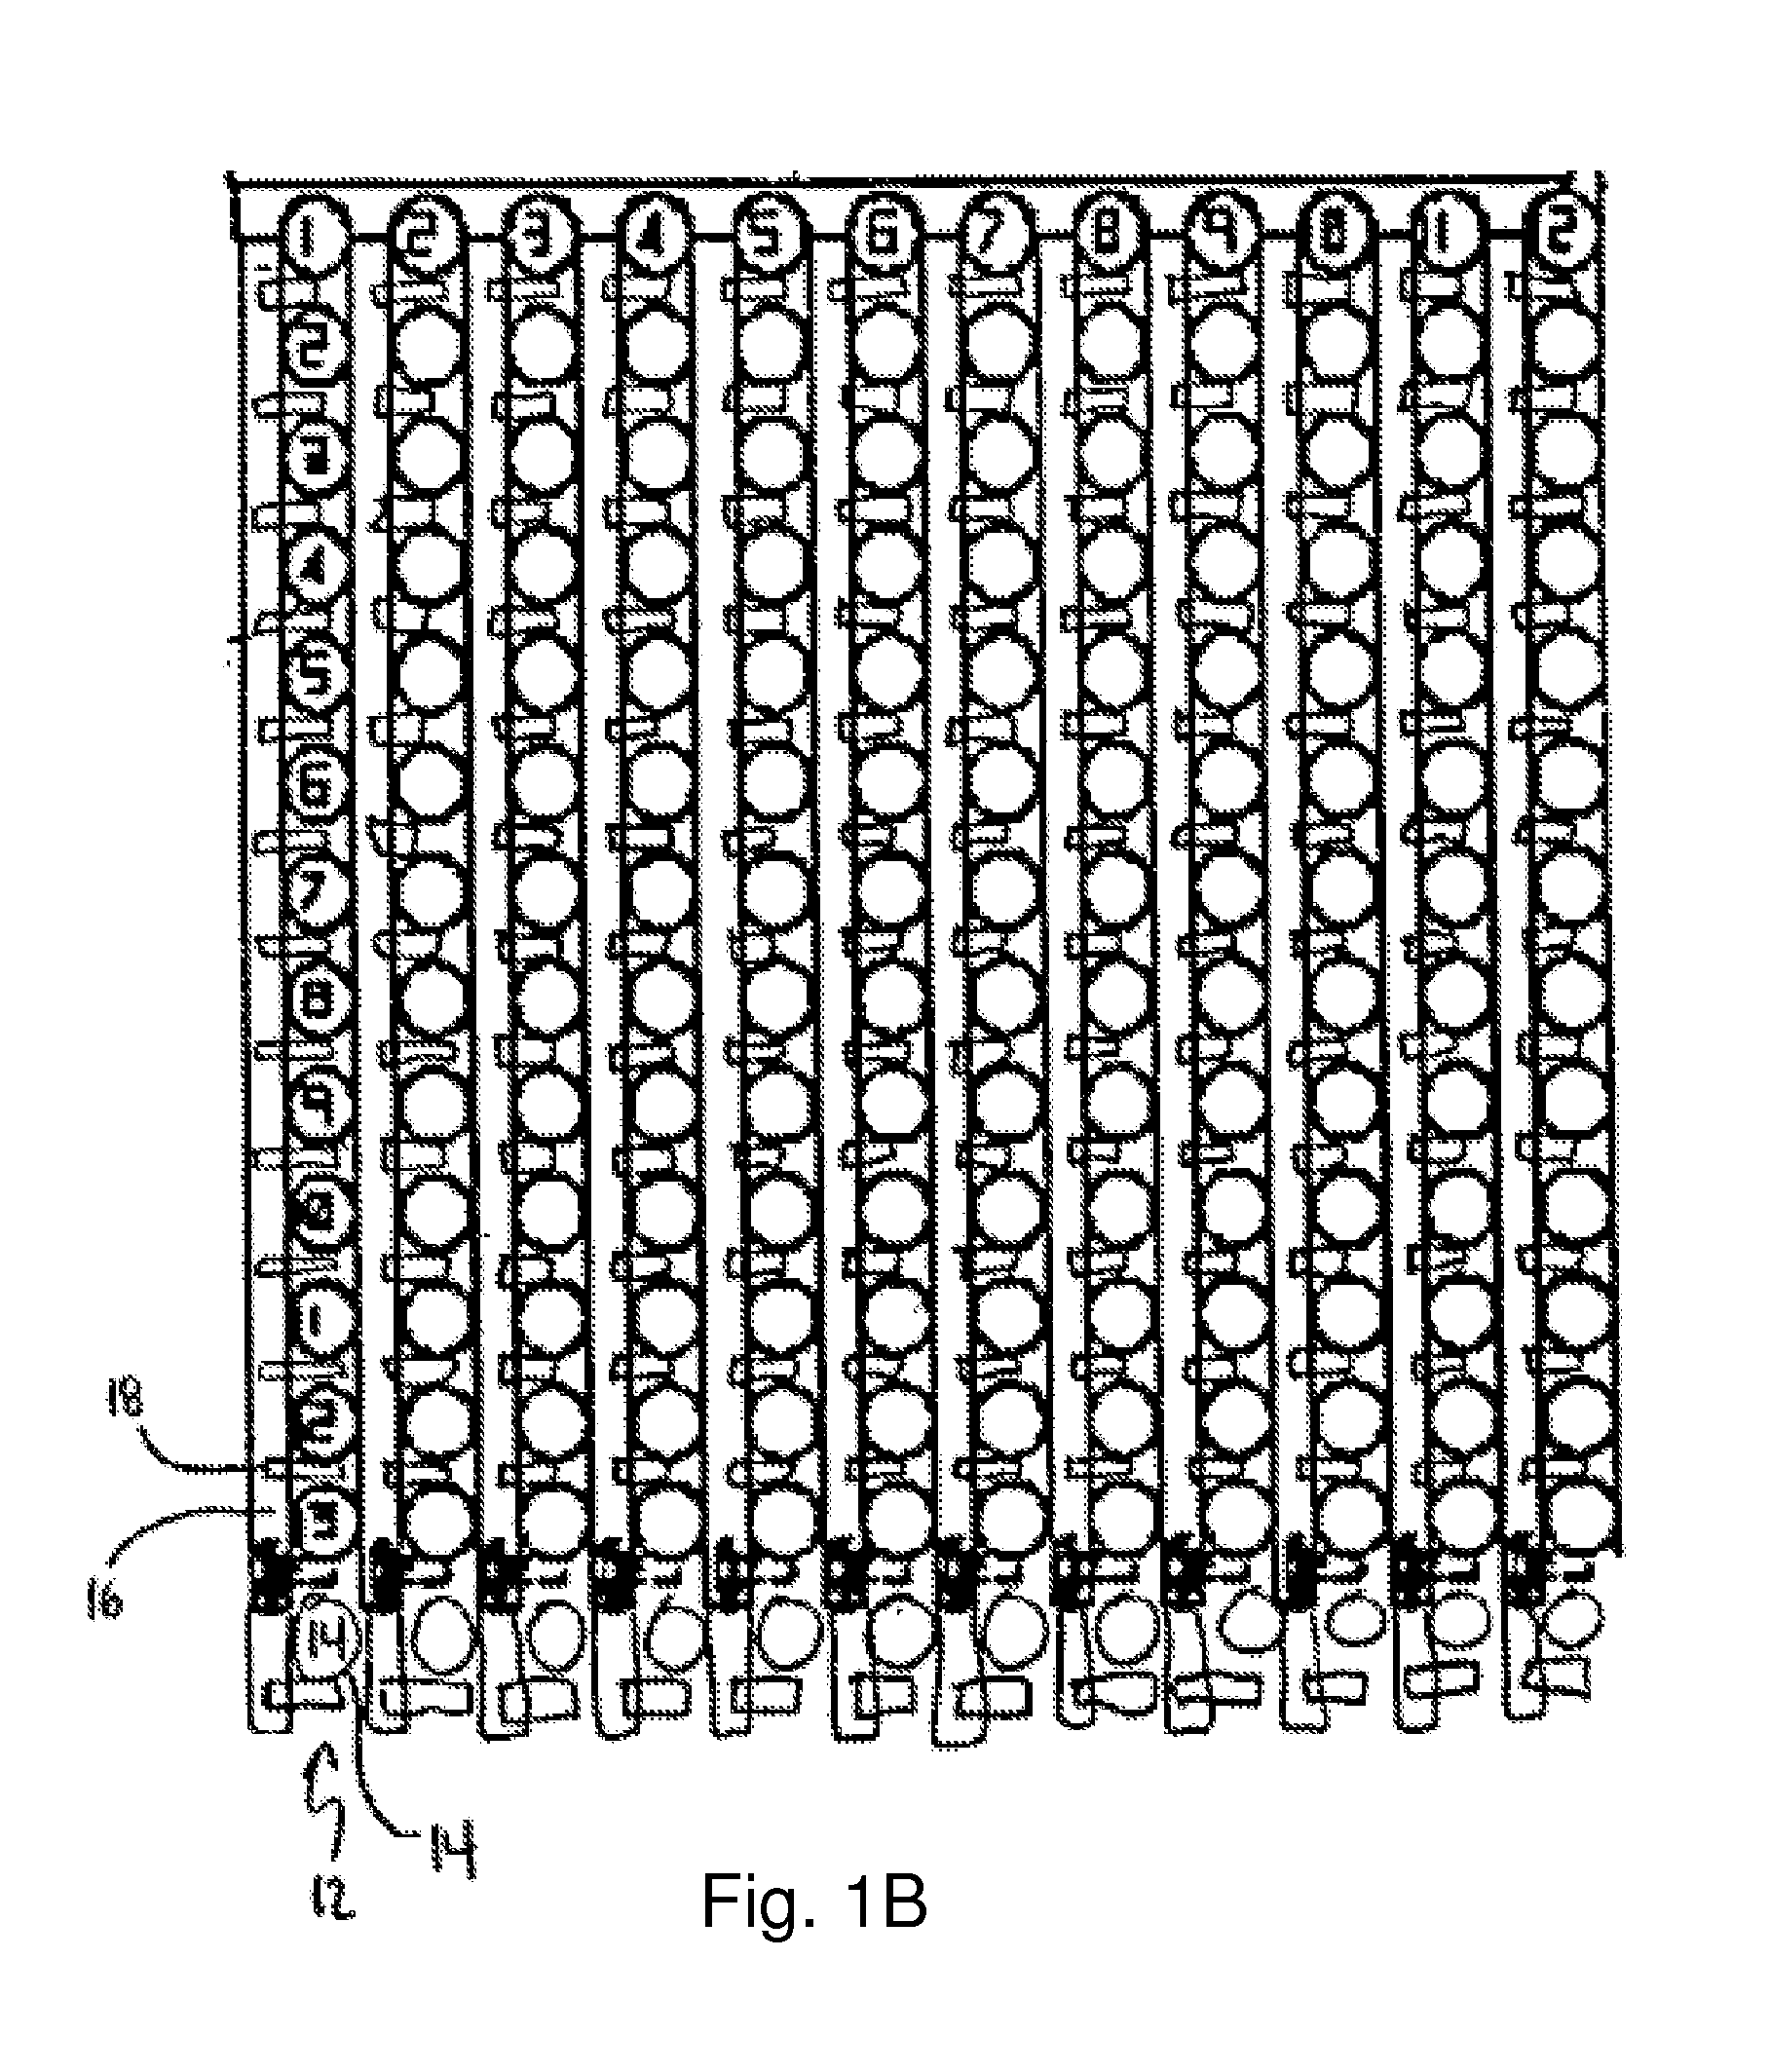
\includegraphics[width=0.8\textwidth]{fig_fb_cells_matrix.png}
    \caption{Diagram of a fingerboard with tubulars. Source:\cite{fig_fb_cells_matrix13}}
    \label{fig:fb_cells_matrix}
\end{figure}
\FloatBarrier

The first patent for a finger board was filed 1929 in the United States, and ever since, new patents that increase their capabilities have been filed. The latest ones use pneumatic cylinders to latch and secure tubulars in place, and a control system managing and tracking the pipes that should be in the fingerboard.

For more information regarding the history of the fingerboard, the reference list of a patent publicized February 2013 by \citet{pat_james13} is suggested. The patent in question discuss a method to report finger position data to the control system. With this feature, the control system becomes aware of its fingers, but knowing if a tubular exists in a given cell requires a fail-free logging of the actions done by other machines.

The goal of this case study is to implement a proof of concept computer vision algorithm to detect tubulars.

\begin{figure}[ht]
    \centering
    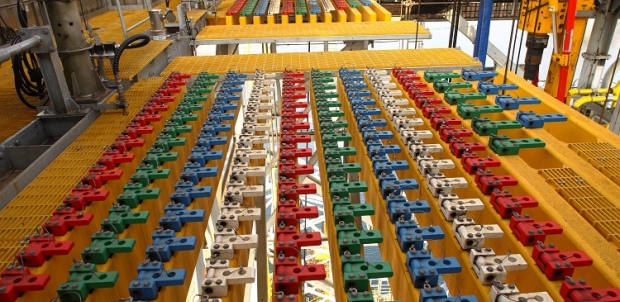
\includegraphics[width=0.8\textwidth]{fingerboard_tsc.jpg}
    \caption{Fingerboard without tubulars. Source:\cite{fig_fb_tsc15}}
    \label{fig:fb_tsc15}
\end{figure}
\FloatBarrier

One possible solution involves using the Hough transform method to find ellipses in the picture, then analyze the region contained within to determine wheter the detected ellipse may outline a tubular. The algorithm implemented in OpenCV is based on a variant called the 2-1 Hough Transform by \citet{yuen90}. Partial occlusion of tubulars are a challenge.

Another more recent method of ellipse detection is presented by \citet{wang14} based on sorted merging. This algorithm is not yet implemented in OpenCV.

\begin{figure}[ht]
    \centering
    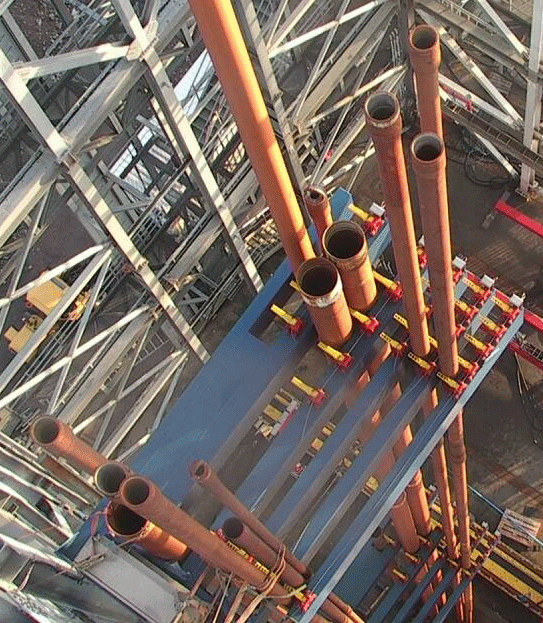
\includegraphics[width=0.8\textwidth]{fb_mhwirth.png}
    \caption{Fingerboard with tubulars. Source: Own work (MHWirth AS)}
    \label{fig:fb_mhwirth}
\end{figure}
\FloatBarrier

